% !Mode:: "TeX:UTF-8"

\chapter{实验过程与结果分析}
\label{experiment}
本章将介绍本项目的实验部分,包括对KITTI数据集、数据预处理、模型训练以及实验结果分析等内容。在结果分析中,我们首先比较DODT各模块对结果的影响,以考察每个模块的有效性;然后我们探讨了关键帧的选取步长对三维物体检测结果的影响,以便确定最优的步长;最后我们也测试了DODT在多目标追踪任务上的性能,并与前沿方法对比。结果显示DODT框架能很好的完成流数据的三维物体检测以及多目标跟踪任务。

\section{KITTI数据集介绍}
\label{kitti}
本项目的所有实验都是基于无人驾驶领域中广泛使用的KITTI公开数据集开展的。KITTI数据集是由德国卡尔斯鲁厄理工学院和丰田美国技术研究院联合采集的,该数据集包含多种传感器数据:一个惯性导航系统(GPS/IMU,型号为OXTS RT 3003)数据,一个激光雷达(Velodyne HDL-64E)数据,两个灰度相机数据(140万像素)以及两个彩色相机数据(140万像素)。其中激光雷达扫描频率为10帧/秒,相机基本与地平面保持平行,图像采集的尺寸为$1382 \times 512$像素。所有传感器的整体布局如\figurename \ref{fig:KITTI}。

\begin{figure}[h]
	\centering
	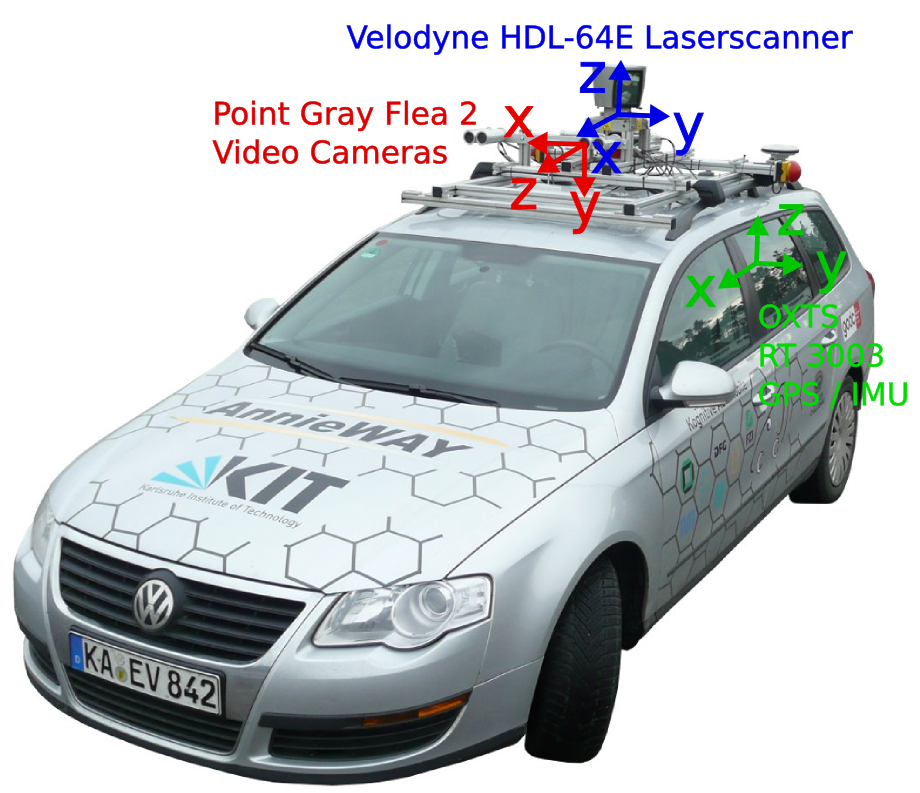
\includegraphics[width=0.6\textwidth]{./imgs/KITTI.png}
	\caption{KITTI数据集传感器整体布局。}
	\label{fig:KITTI}
\end{figure}

KITTI数据集根据不同的任务分为stero、flow、scenceflow、depth、odometry、object以及tracking等部分,对应着场景流估计、深度估计、路径规划、物体检测以及目标追踪等任务。每一个任务数据包都包含了海量的训练数据以及测试数据,供研究者使用。本项目主要使用了KITTI数据集的tracking数据包,该数据包由21段训练视频流(共8004帧数据)以及29段测试视频流(共11095帧数据)组成。每一段视频流都是由连续的RGB图像帧以及三维点云帧组成,在训练数据集中,还包含了每一帧数据对应的二维目标框(针对图像数据)以及三维目标框(针对点云数据)。此外,针对每一段视频流,KITTI还提供了传感器的标定信息以及每一帧的GPS/IMU数据,供研究者数据标定时使用。

多目标追踪的标签共有10项,记录了帧的信息以及帧中每个目标的信息。信息列举如下:
\begin{itemize}
	\item frame id:帧的编号;
	\item object id:每一帧中目标的编号,也是轨迹的编号;
	\item type:目标的类别,有”Car“,”Van“, "Trunk",”Pedestrian“,”Cyclist“等类别,本实验将”Car“和”Van“合并为”Car“类,并只针对”Car“类进行检测和追踪;
	\item truncated:标记目标是否被图像边界截断,”0“表示不截断,”1“表示截断;
	\item occluded:标记目标被遮挡的程度,共有0到3四个取值,”0“表示完全可视,”1“表示部分遮挡,”2“表示大部分遮挡,”3“表示完全遮挡;
	\item alpha:目标的观测角,$\alpha \in [-\pi, \pi]$;
	\item bbox:物体在图像上的2D边界框,包含左上角,右下角的坐标值;
	\item dimensions:物体的高、框和长,单位为米;
	\item location:物体底部中心点在相机坐标系的三维坐标 x,y,z,单位为米;
	\item ry:物体在相机坐标系沿Y轴的旋转角,$r_y \in [-pi, pi]$。
\end{itemize}
其中目标的观测角$\alpha = -[(\pi+r_y) + (\pi+\beta)]$,$r_y$与$\beta$如\figurename \ref{fig:kitti_obj}所示,而目标的location坐标如\figurename \ref{fig:kitti_box3d}所示。
\begin{figure}[!t]
	\centering
	\begin{minipage}[t]{0.5\textwidth}
		\centering
		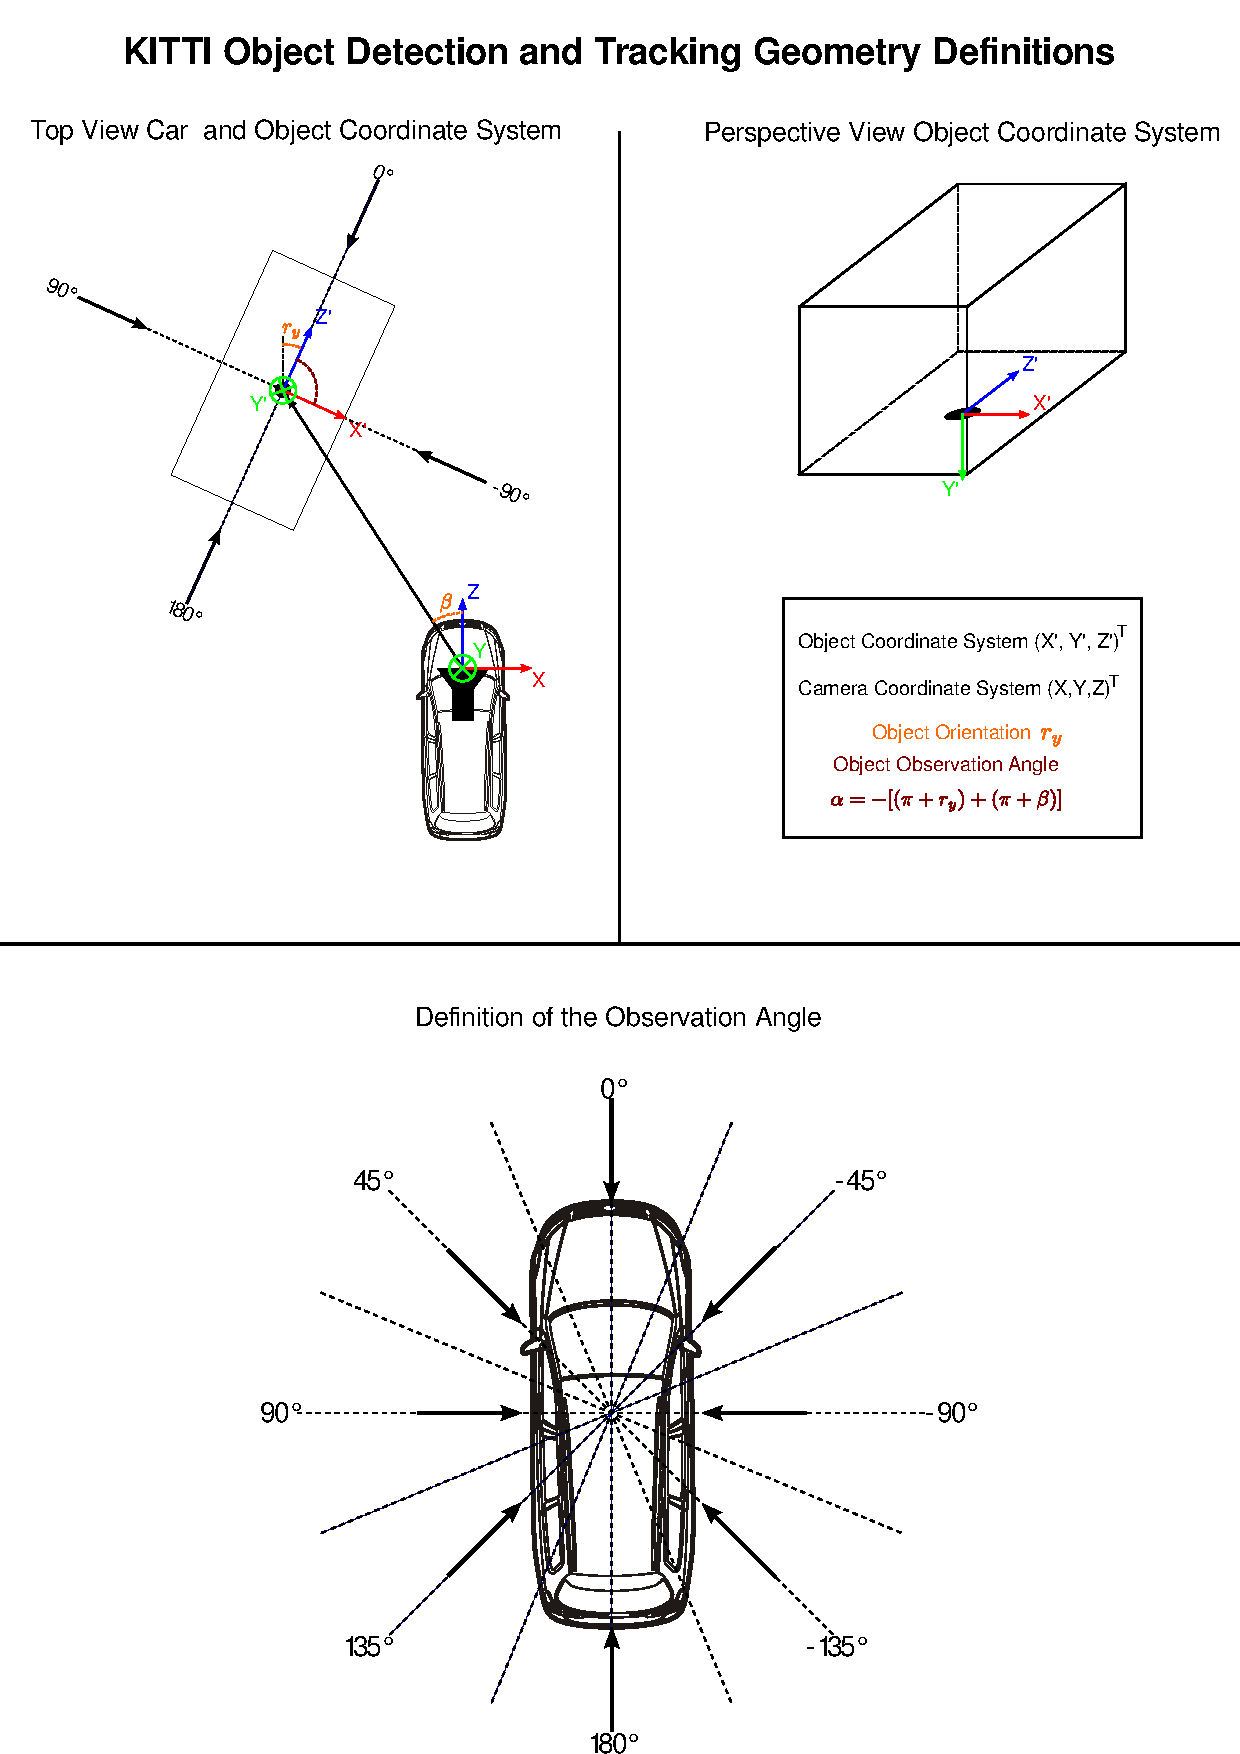
\includegraphics[trim={0cm, 15cm, 12cm, 2.5cm}, clip,width=\textwidth]{./imgs/KITTI_obj.pdf}
		\caption{KITTI数据集观测角与转向角示意图。}
		\label{fig:kitti_obj}
	\end{minipage}
	\begin{minipage}[t]{0.48\textwidth}
		\centering
		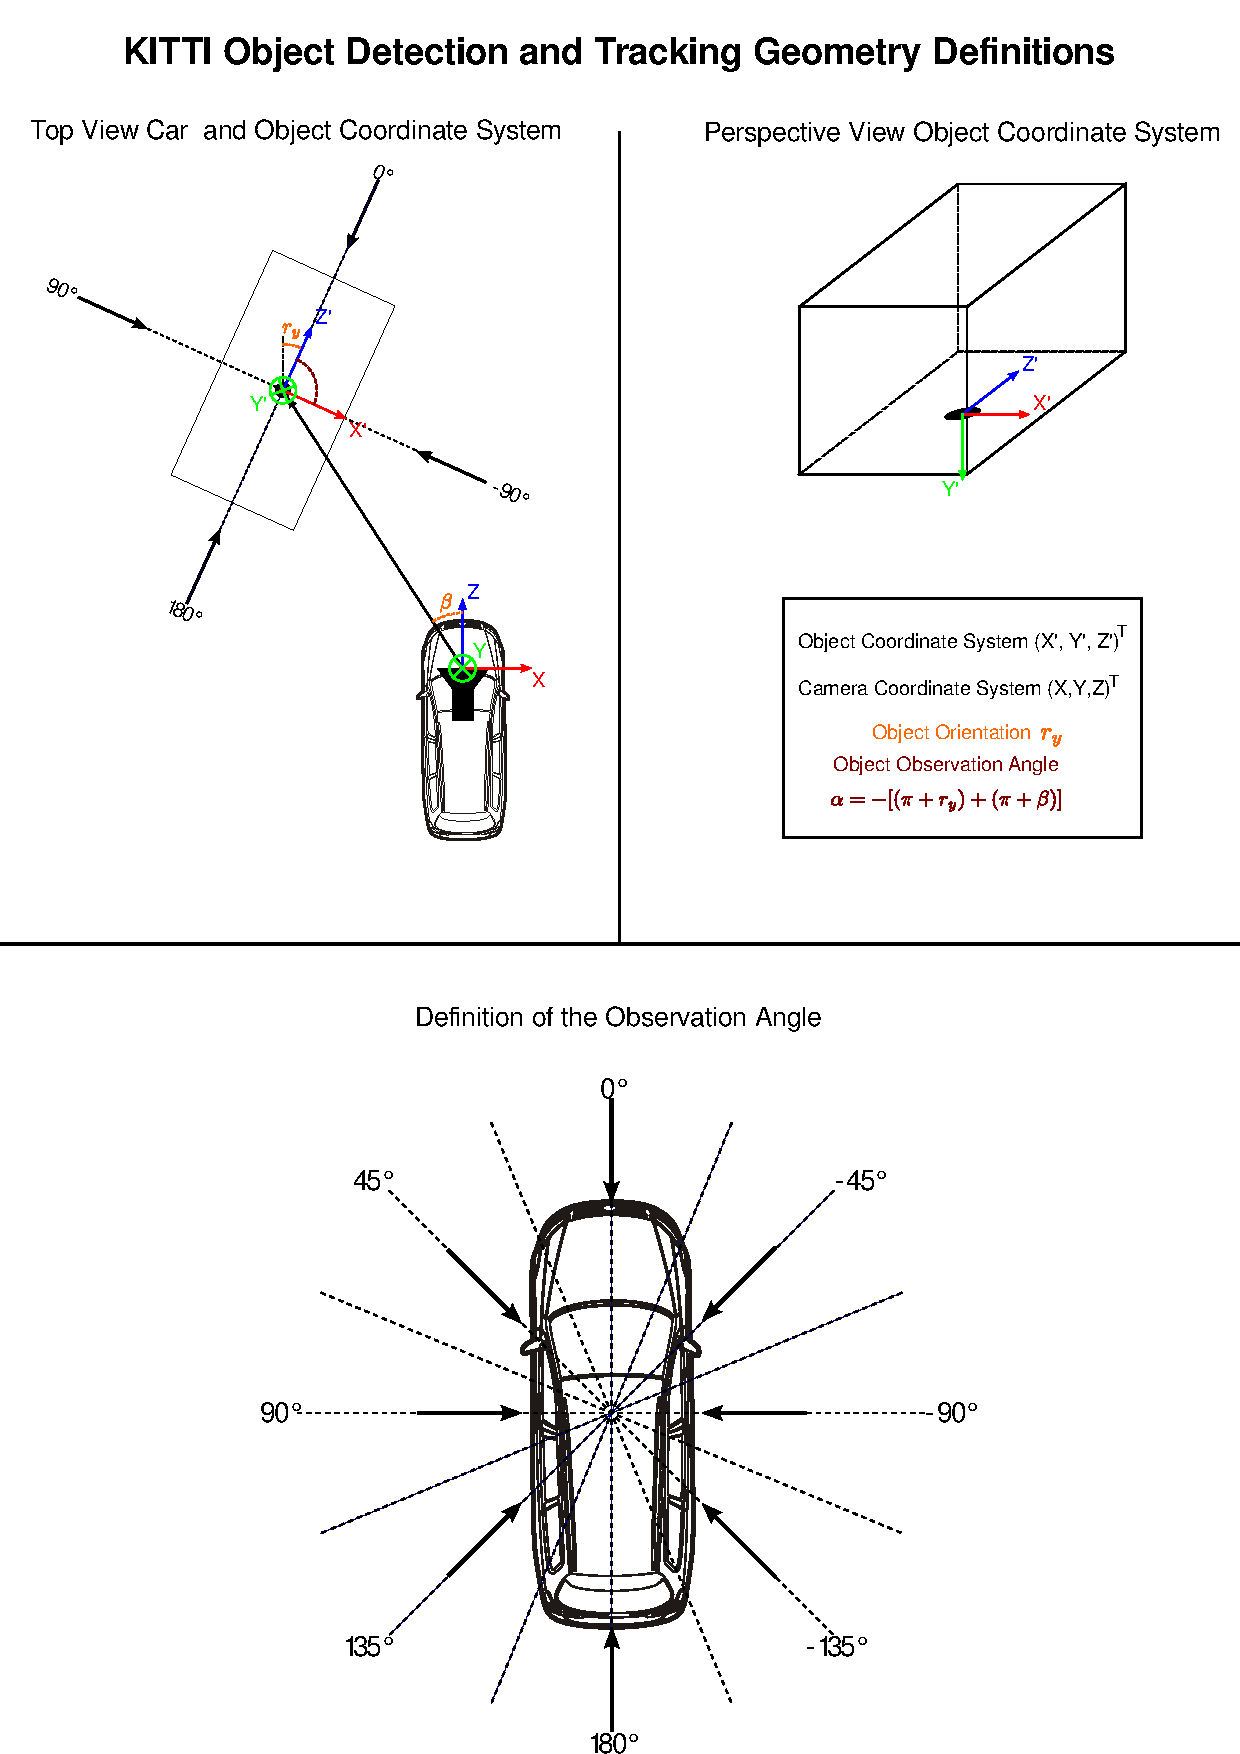
\includegraphics[trim={12cm, 20cm, 1.8cm, 2.5cm}, clip,width=\textwidth]{./imgs/KITTI_obj.pdf}
		\caption{KITTI数据集目标的位置坐标。}
		\label{fig:kitti_box3d}
	\end{minipage}
\end{figure}


传感器的标定信息保存在”calib.txt“文件中,其中包含了相机的参数矩阵以及各传感器之间的旋转矩阵。信息列举如下:
\begin{itemize}
	\item P0-P3:四个相机的内参矩阵 $P \in \mathcal{R}^{3\times 4}$;
	\item R0\_rect:$\mathcal{R}^{3\times 3}$,将摄像机坐标系转换到图像坐标系的校准矩阵;
	\item Tr\_velo\_to\_cam:$\mathcal{R}^{3\times 4}$,激光雷达坐标系到摄像机坐标系的旋转矩阵;
	\item Tr\_imu\_to\_velo:$\mathcal{R}^{3\times 4}$,IMU坐标系到激光雷达坐标系的旋转矩阵。
\end{itemize}

GPS/IMU数据提供了30项信息,其中包含每一帧中自身车辆的经纬度、海拔、三个欧拉角(roll,yaw以及pitch)、速度、加速度、角速度等信息。本实验主要使用到了经纬度以及欧拉角信息将不同帧之间的信息校准到同一坐标系。欧拉角包含了偏航角(yaw,表示机体轴在水平面上的投影与地轴之间的夹角,右偏为正)、俯仰角(pitch,表示机体轴与地平面之间的夹角,抬头为正) 以及翻滚角(roll,表示机体对称面绕机轴转动的角度,右滚为正),如\figurename \ref{fig:euler}所示。
\begin{figure}[t]
	\centering
	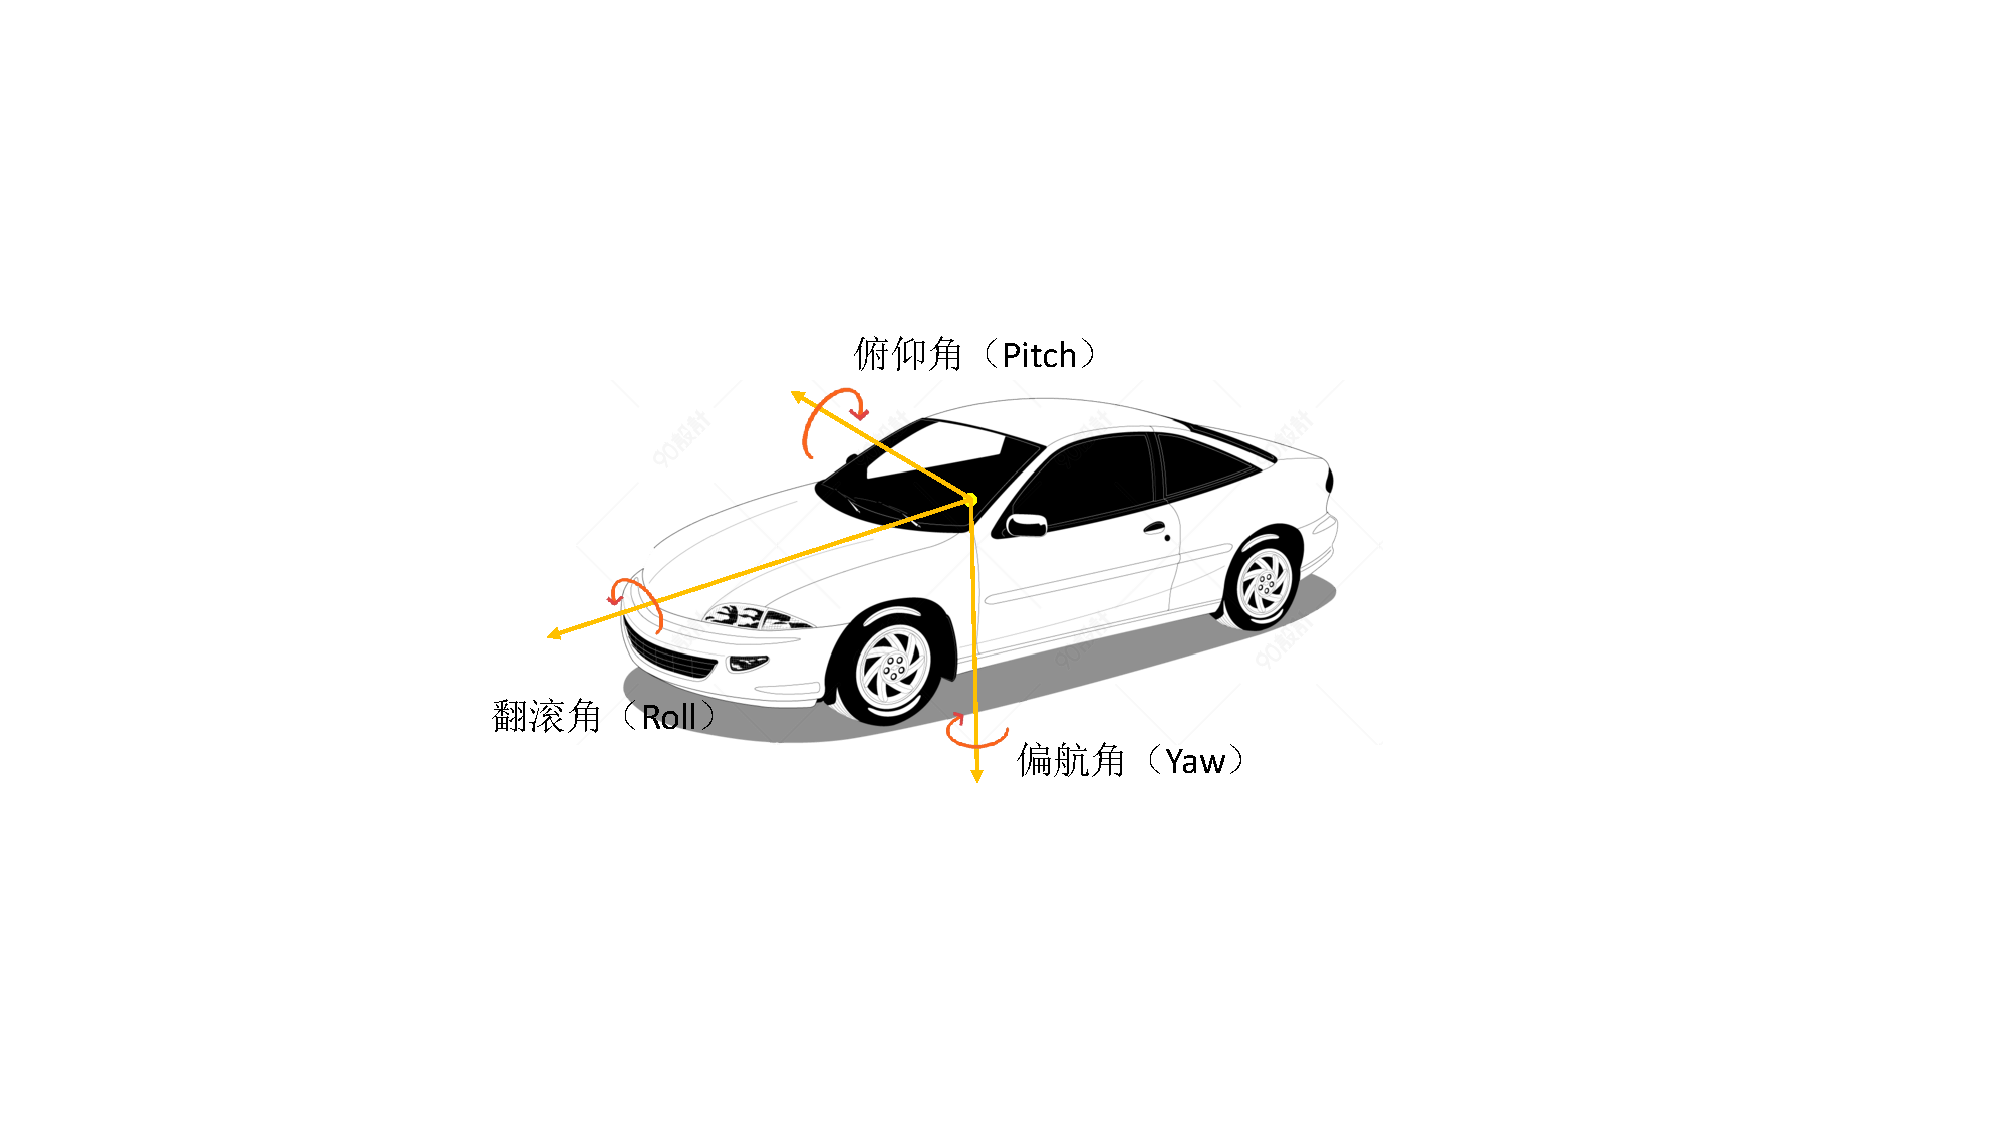
\includegraphics[trim={5cm, 6cm, 5cm, 5cm}, clip,width=\textwidth]{./imgs/euler.pdf}
	\caption{三个欧拉角的方向示意图。}
	\label{fig:euler}
\end{figure}



\section{数据预处理}
\label{preprocessing}


\section{模型训练}
\label{training}


\section{实验结果分析}
\label{results}


\subsection{三维物体检测结果分析}
\label{ablation_study}

\begin{table}[t]
	\centering
	\wuhao
	\caption{候选框预测性能比较。}
	\vspace{0.3cm}
	\begin{tabular}{ccc}
		\toprule[1.5pt]
		方法        & 原始 RPN & \textit{Shared RPN}  \\ \midrule
		准确率(\%)  & 97.81      & \textbf{98.47}       \\
		\bottomrule[1.5pt]
	\end{tabular}
	\label{table:rpn_result}
\end{table}


\begin{table}\centering
	\wuhao
	\caption{DODT的不同设置在验证数据集上的结果(只预测“Car”类别)。每项的指标为$AP_{3D}/AP_{BEV}$ (\%), 为三维物体检测在3D视角和BEV视角的平均精度。 “S” 表示\textit{Shared RPN}模块, “T” 表示时序信息处理模块, “M” 表示运动插值模块。 $\tau$ 是关键帧选取步长。} 
	\vspace{0.3cm}
	\resizebox{\textwidth}{!}{
		\begin{tabular}{ccccccccc}
			\toprule[1.5pt]
			&\multicolumn{1}{c|}{}   & \multicolumn{3}{c|}{IoU = 0.5}  		         & \multicolumn{3}{c|}{IoU = 0.7}          &  \\ \midrule
			\multicolumn{1}{c|}{方法} & \multicolumn{1}{c|}{模块}    & Easy     & Moderate   & \multicolumn{1}{c|}{Hard}     & Easy  & Moderate & \multicolumn{1}{c|}{Hard}    & FPS \\\midrule
			\multicolumn{1}{c|}{AVOD\cite{ku2018joint}}     &\multicolumn{1}{c|}{-}     & 90.13 / 90.91  & 80.00 / 81.79 & \multicolumn{1}{c|}{71.61 / 81.79}  & 76.00 / 90.90 & 57.23 / 81.73 & \multicolumn{1}{c|}{56.13 / 72.69}   & 10.0\\
			\multicolumn{1}{c|}{DODT($\tau$ = 1)}     &\multicolumn{1}{c|}{S}     & 88.28 / 99.97  & 85.74 / 90.90 & \multicolumn{1}{c|}{86.14 / 90.89}  & 83.44 / 90.82 & 67.48 / 90.79 & \multicolumn{1}{c|}{61.24 / 90.80}     & 6.7 \\
			\multicolumn{1}{c|}{DODT($\tau$ = 1)}     &\multicolumn{1}{c|}{S+T}     & 88.32 / \textbf{99.99}  & 86.53 / 90.90 & \multicolumn{1}{c|}{86.71 / \textbf{90.90}}  & 83.60 / 90.82 & 68.93 / 90.80 & \multicolumn{1}{c|}{62.69 / 90.81}   & 5.9\\
			\multicolumn{1}{c|}{DODT($\tau$ = 1)}     &\multicolumn{1}{c|}{S+M}     & 89.99 / 99.95  & 87.86 / 90.87 & \multicolumn{1}{c|}{87.81 / 90.86}  & 86.89 / 90.89 & 73.96 / 90.83 & \multicolumn{1}{c|}{67.07 / 81.79}   & 6.5\\
			\multicolumn{1}{c|}{DODT($\tau$ = 1)}     &\multicolumn{1}{c|}{S+T+M} & \textbf{90.63} / 99.95  & 89.07 / 90.90 & \multicolumn{1}{c|}{88.79 / \textbf{90.90}}  & 88.74 / 90.91 & 75.27 / 90.84 & \multicolumn{1}{c|}{68.75 / 90.57}   & 5.7\\ \midrule
			\multicolumn{1}{c|}{DODT($\tau$ = 2)}     &\multicolumn{1}{c|}{S+T+M} & 90.60 / 99.94  & \textbf{89.19 / 90.91} & \multicolumn{1}{c|}{\textbf{88.91} / 90.88}  & \textbf{88.90 / 90.92} & \textbf{76.64} / 90.85 & \multicolumn{1}{c|}{75.81 / 90.83}   & 8.6\\
			\multicolumn{1}{c|}{DODT($\tau$ = 3)}     &\multicolumn{1}{c|}{S+T+M} & 90.61 / 99.98  & 89.01 / 90.89 & \multicolumn{1}{c|}{88.84 / 90.89}  & 88.81 / 90.91 & 76.38 / \textbf{90.86} & \multicolumn{1}{c|}{\textbf{75.83 / 90.85}}   & 11.4\\
			\multicolumn{1}{c|}{DODT($\tau$ = 4)}     &\multicolumn{1}{c|}{S+T+M} & 90.55 / 99.94  & 88.82 / 90.88 & \multicolumn{1}{c|}{88.34 / 90.87}  & 88.43 / 90.91 & 75.70 / 90.82 & \multicolumn{1}{c|}{68.75 / 90.82}   & 14.3\\
			\multicolumn{1}{c|}{DODT($\tau$ = 5)}     &\multicolumn{1}{c|}{S+T+M} & 87.98 / 90.91  & 85.57 / 90.87 & \multicolumn{1}{c|}{86.01 / 90.87}  & 81.59 / 90.81 & 67.30 / 90.76 & \multicolumn{1}{c|}{61.35 / 81.73}   & 17.1\\
			\multicolumn{1}{c|}{DODT($\tau$ = 6)}     &\multicolumn{1}{c|}{S+T+M} & 78.77 / 90.75  & 70.88 / 90.71 & \multicolumn{1}{c|}{71.65 / 81.70}  & 71.71 / 90.44 & 55.86 / 81.50 & \multicolumn{1}{c|}{56.80 / 81.51}   & \textbf{20.0} \\ 
			\bottomrule[1.5pt]
	\end{tabular}}
	\label{table:result_detection}
\end{table}




\subsection{流数据检测结果分析}
\label{stream_result}

\begin{figure}[!t]
	\centering
	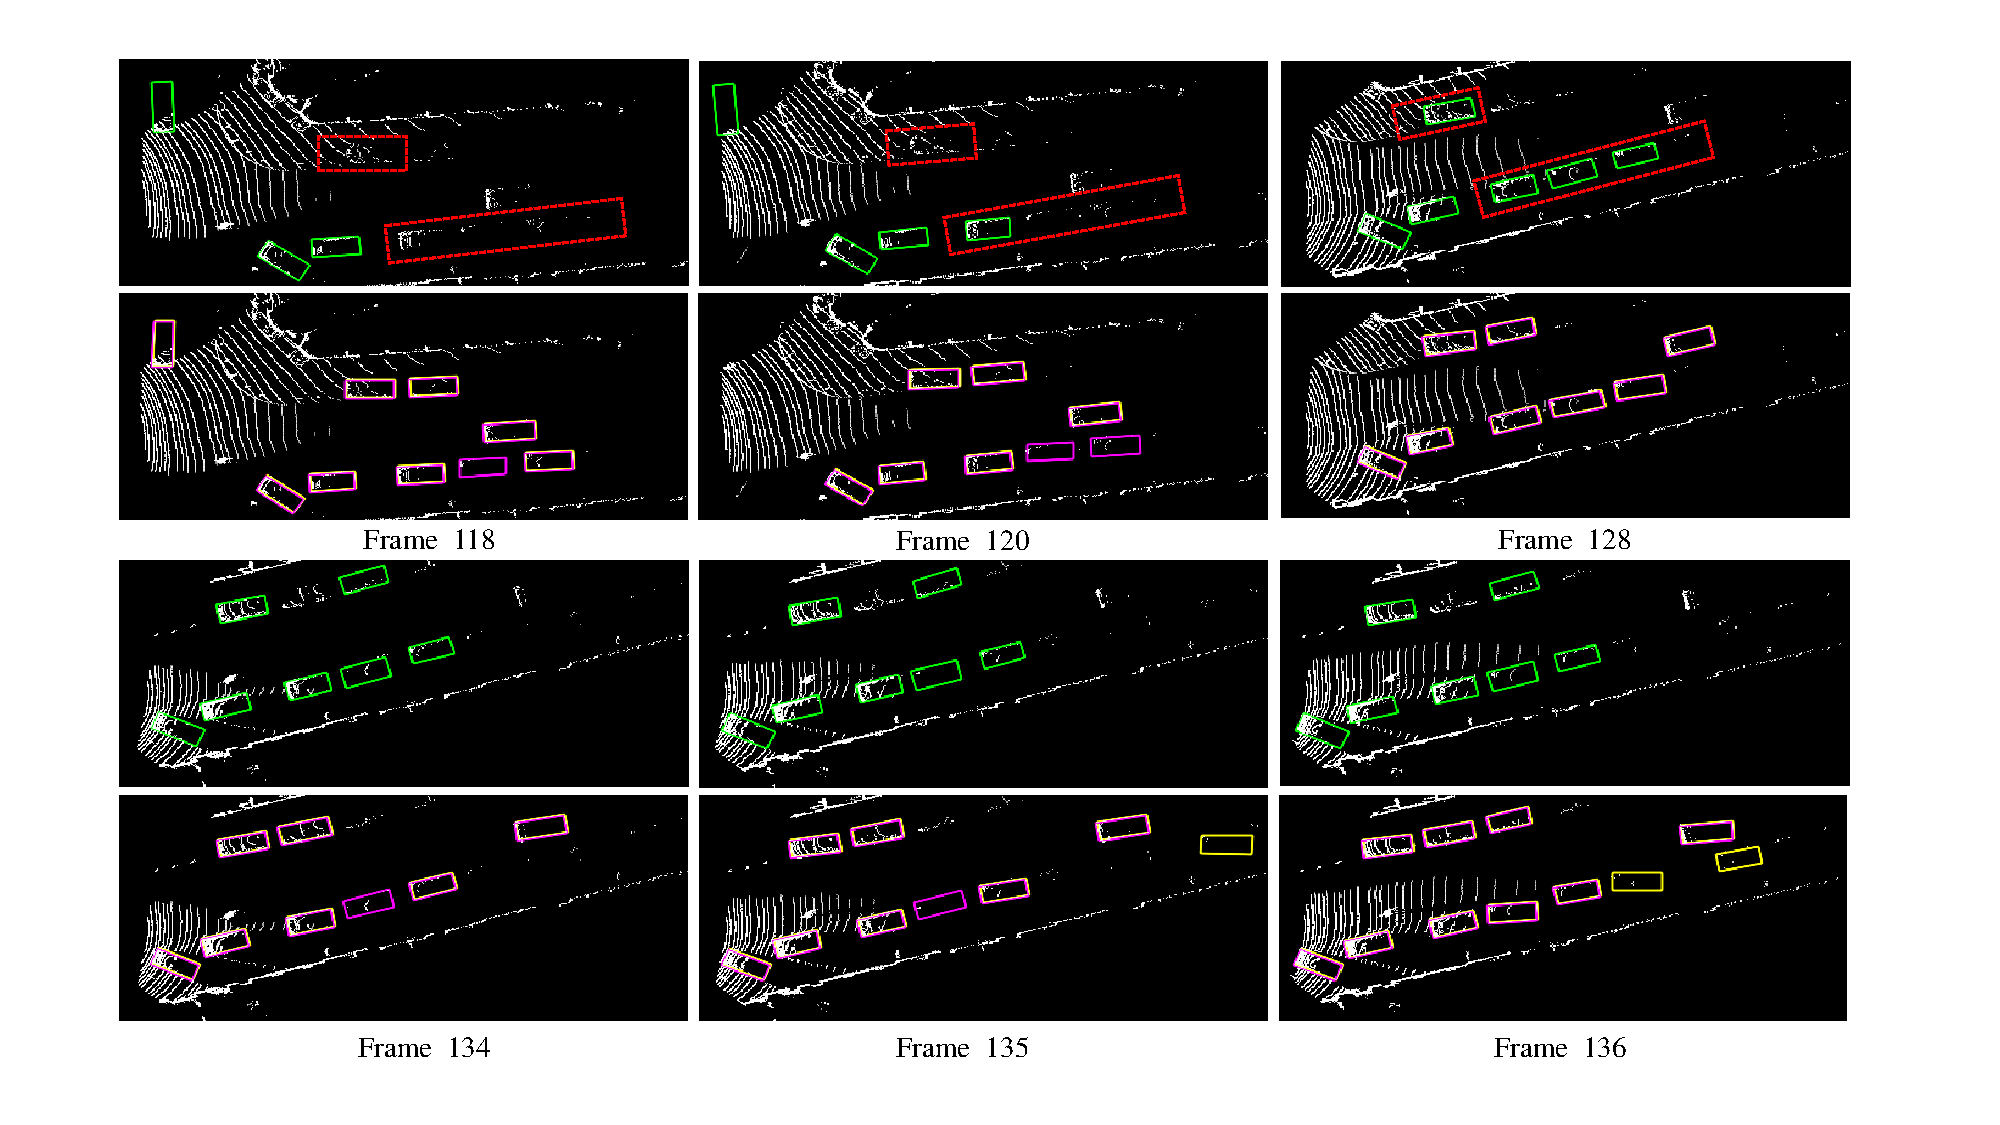
\includegraphics[trim={2cm, 1cm, 2.5cm, 1cm}, clip, width=\textwidth]{./imgs/examples.pdf}
	\vspace{-1.0cm}
	\caption{视频序列0的标签以及预测结果可视化。\textcolor{green}{绿色}为官方提供的标签框, \textcolor{yellow}{黄色}是时序步长$\tau = 1$的预测结果,\textcolor{magenta}{洋红色}为时序步长$\tau = 3$的预测结果。混合颜色的框是黄色框和洋红色框重叠造成的,该结果最好彩色打印查看。}
	\label{fig:examples}
\end{figure}


\subsection{多目标跟踪实验分析}
\label{mot_result}

\begin{table}
	\centering
	\wuhao
	\caption{DODT的不同设置在KITTI多目标追踪验证数据集上的结果。S 表示\textit{Shared RPN}模块, T 表示时序信息处理模块, M 表示运动插值模块。 $\tau$ 是关键帧选取时间步长。}
	\vspace{0.3cm}
	\resizebox{\textwidth}{!}{
		\begin{tabular}{cccccccc}
			\toprule[1.5pt]
			方法   & 模块 & MOTA(\%)$\uparrow$ & MOTP(\%)$\uparrow$ & MT(\%)$\uparrow$ & ML(\%)$\downarrow$ & IDS$\downarrow$&  FM$\downarrow$ \\ \midrule
			AVOD\cite{ku2018joint}    & -      & 66.05    & 82.97    & 46.22  & 12.18  & \textbf{2}      &  113  \\
			DODT($\tau$ = 3)          & S      & 76.53    & \textbf{83.93}    & 68.91  & 7.14   & 32      &  80  \\
			DODT($\tau$ = 3)          & S+T      & 77.52    & 83.75    & 69.33  & 7.56   & 37     &  77  \\
			DODT($\tau$ = 3)          & S+M      & 78.73    & \textbf{83.93}    & 68.49  & 9.55   & \textbf{2}      &  \textbf{48}  \\
			DODT($\tau$ = 3)  & S+T+M    & \textbf{79.72}   & 83.55    & \textbf{71.85}  & \textbf{5.46}  & 7  &  66  \\ 
			\bottomrule[1.5pt]
	\end{tabular}}
	\label{table:result_tracking}
\end{table}


\begin{table}
	\centering
	\wuhao
	\resizebox{\textwidth}{!}{
		\begin{tabular}{cccccccc}
			\toprule[1pt]
			方法    & MOTA(\%)$\uparrow$ & MOTP(\%)$\uparrow$ & MT(\%)$\uparrow$ & ML(\%)$\downarrow$ & IDS$\downarrow$&  FM$\downarrow$ &FPS$\uparrow$ \\ \midrule
			DSM\cite{frossard2018end}                         & 76.15    & 83.42    & 60.00  & 8.31  & 296  & 868  & 10.0 (GPU)  \\ %DSM
			3DT\cite{Hu3DT19} 	                              & \textbf{84.52}    & \textbf{85.64}	& \textbf{73.38}  & \textbf{2.77}  & 377  & 847  & 33.3 \\ %3DT
			Complexer-YOLO\cite{Simon_2019_CVPR_Workshops}    & 75.70    & 78.46    & 58.00  & 5.08  & 1186 & 2096 & \textbf{100.0} \\ %Complexer-YOLO
			3D-CNN/PMBM\cite{scheidegger2018mono}             & 80.39    & 81.26	& 62.77  & 6.15  & 121  & 613  & 71.4 \\  %3D-CNN/PMBM
			DODT(ours)                                        & 76.68    & 81.65    & 60.77  & 11.69 & \textbf{63}   & \textbf{384}  & 76.9 \\ 
			\bottomrule[1pt]
	\end{tabular}}
	\caption{DODT与现有的前沿方法在KITTI三维多目标追踪公开排行榜中的对比。FPS的计算不包含目标检测时间。}
	\label{label:result_kitti}
\end{table}



\section{结果展示}
\label{show}

\section{本章总结}
\label{exp_conclusion}


% 打印时插入必要的空白页
\ifprint
	\newpage
	\thispagestyle{empty}
	\mbox{}
	
	% 避免空白页影响页码编号
	\clearpage
	\setcounter{page}{10}
\fi